\documentclass[12pt]{article}
\usepackage[spanish]{babel}
\usepackage{geometry}
\geometry{a4paper, margin=1in}
\usepackage{graphicx}
\usepackage{xcolor}
\usepackage{titlesec}
\usepackage{parskip}
\usepackage{multicol}
\usepackage{cite}
\usepackage{float}

\definecolor{highlight}{RGB}{255, 255, 0}

\titleformat{\section}{\normalfont\Large\bfseries}{\thesection}{1em}{}
\titleformat{\subsection}{\normalfont\large\bfseries}{\thesubsection}{1em}{}

\begin{document}

% Logos
\begin{minipage}{0.45\textwidth}
    
\includegraphics[width=0.4\textwidth]{inFiles/Figures/epnLogo.jpg}
\end{minipage}
\hfill
\begin{minipage}{0.45\textwidth}
    \raggedleft
    
\includegraphics[width=0.4\textwidth]{inFiles/Figures/FIS_logo.jpg}
\end{minipage}

\vspace{0.5cm}

% Títulos principales
\begin{center}
    \textbf{ESCUELA POLITÉCNICA NACIONAL}\\[0.2cm]
    \textbf{FACULTAD DE INGENIERÍA DE SISTEMAS}\\[0.2cm]
    \textbf{INGENIERÍA {\textbf{EN COMPUTACIÓN}}}
\end{center}

\vspace{0.5cm}
\hrule
\vspace{0.5cm}

% Datos principales
\noindent\textbf{PERÍODO ACADÉMICO:} 2025-A\\[0.2cm]
\noindent\textbf{ASIGNATURA:} ICCD412 Métodos Numéricos \hfill \textbf{GRUPO:} GR2\\[0.2cm]
\noindent\textbf{TIPO DE INSTRUMENTO:} Tarea 7\\[0.2cm]
\noindent\textbf{FECHA DE ENTREGA LÍMITE:} 11/05/2025\\[0.2cm]
\noindent\textbf{ALUMNO:} Murillo Tobar Juan

\vspace{0.5cm}
\hrule
\vspace{1cm}


% Secciones
\section*{TEMA}
Método de Newton, Secante y Posición Falsa

\vspace{0.5cm}

\section*{OBJETIVOS}
\begin{itemize}
    \item Comprender y comparar las similitudes y diferencias entre los 3 métodos.
    \item Analizar porque un método cerrado como lo es la posición falsa es mejor que los dos métodos abiertos mencionados en este documento.

\end{itemize}

\vspace{0.5cm}

\section*{MARCO TEÓRICO}

\textbf{Método de la posición falsa}
\normalsize\newline\newline
Es un método que rescata las mejores características del método de bisección y del método de la secante. 
Como se menciona en \cite{sauer2013analisis} es muy similar al método de bisección porque es un método encerrado pero reemplaza el punto medio por un método secante. 
También denominado Regula Falsi este método pareciera que es mejor que el método de bisección pero en realidad su convergencia es mucho mas lenta porque no cubre la mitad de los subintervalos generados como lo hace el método de bisección.
\vspace{0.5cm}

\section*{DESARROLLO}
\large\textbf{CONJUNTO DE EJERCICIOS 2.3}
\normalsize\newline
\textbf{1}. Sea $f(x) = x^2 - 6$ y $p_0 = 1$. Use el método de Newton para encontrar $p_2$.

Sabemos que $f'(x) = 2x$ y mediante la formula de este método obtenemos los siguientes resultados.


\begin{center}
    \begin{tabular}{|c|c|c|c|}
        \hline
        $p$&$X$&$X_{n-1}$&$E_{est}$\\
        \hline
        0 & 1&  & \\
        1 &$ 3.5$& 1&2.25\\
        2 & 2.607143& 3.5&0.8928\\
        \hline
      \end{tabular} 
\end{center}


\textbf{2}.Sea $f(x) = -x^3 - \cos(x)$ y $p_0 = -1$. Use el método de Newton para encontrar $p_2$. ¿Se podría usar $p_0$ = 0?

\begin{figure}[H]
    \centering
    \begin{minipage}{0.5\textwidth}
        \centering
        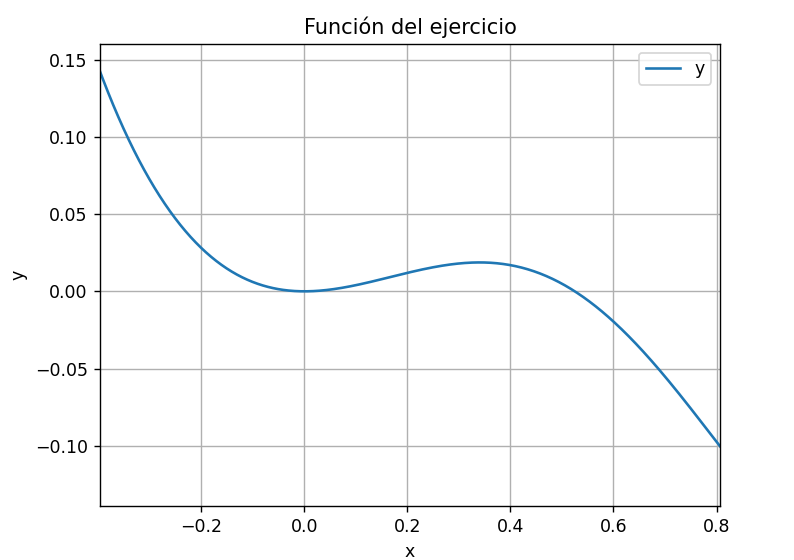
\includegraphics[width=0.9\textwidth]{./inFiles/Figures/Cap1.png}
        \caption{Gráfica \( y = -x^3 - \cos(x) \)}
    \end{minipage}
\end{figure}

Sabemos que $f'(x) = -3x^2 + \sen(x)$ y mediante la formula de este método obtenemos los siguientes resultados.


\begin{center}
    \begin{tabular}{|c|c|c|c|}
        \hline
        $p$&$X$&$X_{n-1}$&$E_{est}$\\
        \hline
        0 & -1&  & \\
        1 &$-0.8803328996$& -1&0.11967\\
        2 &$-0.8656841632$&$-0.8803328996$&0.01465\\
        \hline
      \end{tabular} 
\end{center}


Y en respuesta si se puede usar como aproximación inicial a 0 es no, ya que, en ese punto la derivada es 0 y por lo tanto resultaría en una indeterminación si usamos el método de Newton.

\textbf{3}.Use el método de Newton para encontrar soluciones precisas dentro de $10^{-4}$ para los siguientes problemas.
(Usando 6 cifras decimales)

\textbf{3.a} $x^3 - 2x^2 - 5 = 0, [1,4]$ 

$p_0 = 2.5$

$f'(x) = 3x^2 -4x$

\begin{center}
    \begin{tabular}{|c|c|c|c|}
        \hline
        $p$&$X$&$X_{n-1}$&$E_{est}$\\
        \hline
        0 & 2.5&  & \\
        1 &$2.714286$&2.5&0.2142\\
        2 &$2.690952$&$2.714286$&0.0233\\
        2 &$2.690647$&$2.690952$&0.000305\\
        \hline
      \end{tabular} 
\end{center}



\textbf{3.b} $x^3 + 3x^2 - 1 = 0, [-3, -2]$ 

$p_0 = -1$

$f'(x) = 3x^2 +6x$

\begin{center}
    \begin{tabular}{|c|c|c|c|}
        \hline
        $p$&$X$&$X_{n-1}$&$E_{est}$\\
        \hline
        0 & -1&  & \\
        1 &$-0.666667$&-1&0.3333\\
        2 &$-0.652778$&$-0.666667$&0.0139\\
        \hline
      \end{tabular} 
\end{center}

\textbf{3.c} $x - \cos(x)=0, [0, \frac{\pi}{2}]$ 

$p_0 = \frac{\pi}{4}$

$f'(x) = 1 + \sen(x)$

\begin{center}
    \begin{tabular}{|c|c|c|c|}
        \hline
        $p$&$X$&$X_{n-1}$&$E_{est}$\\
        \hline
        0 & $\frac{\pi}{4}$&  & \\
        1 &$0.739536$&$\frac{\pi}{4}$&0.0459\\
        2 &$0.739085$&$0.739536$&0.0000451\\
        \hline
      \end{tabular} 
\end{center}


\textbf{3.d} $x - 0.8 -0.2\sen(x) = 0, [0, \frac{\pi}{2}]$ 

$p_0 = \frac{\pi}{4}$

$f'(x) = 1 - 0.2\cos(x)$

\begin{center}
    \begin{tabular}{|c|c|c|c|}
        \hline
        $p$&$X$&$X_{n-1}$&$E_{est}$\\
        \hline
        0 & $\frac{\pi}{4}$&  & \\
        1 &$0.964335$&$\frac{\pi}{4}$&0.1789\\
        2 &$0.964333$&$0.964335$&0.002786\\
        \hline
      \end{tabular} 
\end{center}


\textbf{4}.Use los tres métodos en esta sección para encontrar las soluciones dentro de $10^{-5}$ para los siguientes
problemas

\textbf{4.a} $3x - e^x = 0$  para $ 1\leq x\leq 2$ 

\textbf{Método de la posición falsa}
\normalsize

\begin{center}
    \begin{tabular}{|c|c|c|c|c|}
        \hline
        $X_n$&$f(X_n)$&$sgn(f(X_n))$&$E_{est}$\\
        \hline
        1        &0.281718& +1& \\
        2        &$-1.389056$&-1&1\\
        1.168615 &0.288312&+1&0.831\\
        1.311516 &0.222751&+1&0.143\\
        1.406664 &0.137677&+1&0.095\\
        1.460170 &0.073818&+1&0.054\\
        1.487410 &0.036611&+1&0.027\\
        1.500573 &0.017461&+1&0.013\\
        1.506773 &0.008172&+1&0.0062\\
        1.509657 &0.003793&+1&0.0028\\
        1.510992 &0.001752&+1&0.0001\\
        1.511608 &0.000808&+1&0.0006\\
        1.511891 &0.000374&+1&0.0002\\
        1.512022 &0.000172&+1&0.0001\\
        1.512082 &0.000080&+1&0.00006\\
        1.512110 &0.000038&+1&0.00003\\
        \hline
      \end{tabular} 
\end{center}


\textbf{Método de la secante}
\normalsize


\begin{center}
    \begin{tabular}{|c|c|c|c|c|}
        \hline
        $X_n$&$f(X_n)$&$E_{est}$\\
        \hline
        1        &0.281718& \\
        2        &$-1.389056$&1\\
        1.168615 &0.288312&0.831\\
        1.311516 &0.222751&0.143\\
        1.797043 &-0.64066&0.095\\
        1.436778 &0.103216&0.054\\
        1.486766 &0.037528&0.027\\
        1.515326 &0.004926&0.013\\
        1.512012 &0.000188&0.0062\\
        \hline
      \end{tabular} 
\end{center}

\textbf{Método de Newton}
\normalsize

$p_0 = 1.5$

$f'(x) = 3 - e^x$

\begin{center}
    \begin{tabular}{|c|c|c|c|}
        \hline
        $p$&$X$&$X_{n-1}$&$E_{est}$\\
        \hline
        0 & $1.5$&  & \\
        1 &$1.512358$&$1.5$&0.0124\\
        2 &$1.512135$&$1.512358$&0.000223\\
        \hline
      \end{tabular} 
\end{center}




\textbf{4.b} $2x + 3\cos(x)  - e^x = 0$  para $ 1\leq x\leq 2$ 

\textbf{Método de la posición falsa}
\normalsize

\begin{center}
    \begin{tabular}{|c|c|c|c|c|}
        \hline
        $X_n$&$f(X_n)$&$sgn(f(X_n))$&$E_{est}$\\
        \hline
        1        &0.902625& +1& \\
        2        &-4.637497&-1&1\\
        1.162925 &0.316541&+1&0.837\\
        1.216410 &0.098815&+1&0.053\\
        1.232758 &0.029748&+1&0.016\\
        1.237648 &0.008860&+1&0.00489\\
        1.239059 &0.002813&+1&0.00141\\
        1.239520 &0.000836&+1&0.00046\\
        1.239657 &0.000248&+1&0.00014\\
        1.239697 &0.000076&+1&0.00004\\
        \hline
      \end{tabular} 
\end{center}

\textbf{Método de la secante}
\normalsize

\begin{center}
    \begin{tabular}{|c|c|c|c|c|}
        \hline
        $X_n$&$f(X_n)$&$E_{est}$\\
        \hline
        1        &0.902625& \\
        2        &-4.637497&1\\
        1.162925 &0.316541&0.84\\
        1.216410 &0.098815&0.053\\
        1.240684 &-0.00416&0.024\\
        1.239703 &0.00005&0.000981\\
        \hline
      \end{tabular} 
\end{center}

\textbf{Método de Newton}
\normalsize

$p_0 = 1.5$

$f'(x) = 2 - 3sen(x) - e^x$

\begin{center}
    \begin{tabular}{|c|c|c|c|}
        \hline
        $p$&$X$&$X_{n-1}$&$E_{est}$\\
        \hline
        0 & $1.5$&  & \\
        1 &$1.268097$&$1.5$&0.23\\
        2 &$1.240119$&$1.268097$&0.028\\
        3 &$1.239714$&$1.240119$&0.000405\\
        \hline
      \end{tabular} 
\end{center}



\textbf{5}.El polinomio de cuarto grado
$$
f(x) = 230x^4 + 18x^3 + 9x^2 - 221x - 9
$$

tiene dos ceros reales, uno en [-1,0] y el otro en [0,1]. Intente aproximar estos ceros dentro de $10^{-6}$ con

\textbf{5a}. El método de posición falsa

\begin{center}
    \begin{tabular}{|c|c|c|c|c|}
        \hline
        $X_n$&$f(X_n)$&$sgn(f(X_n))$&$E_{est}$\\
        \hline
        0        &-9& -1& \\
        -0.05    &2.0717&+1&0.05\\
        -0.0594  &4.1582&+1&0.0094\\
        -0.04062 &-0.0087&-1&0.02\\
        \hline
      \end{tabular} 
\end{center}

\begin{center}
    \begin{tabular}{|c|c|c|c|c|}
        \hline
        $X_n$&$f(X_n)$&$sgn(f(X_n))$&$E_{est}$\\
        \hline
        0.8     &-76.616& -1& \\
        1       &27     &+1&0.2\\
        0.9479  &-9.3832&-1&0.05\\
        0.96134 &-0.7038&-1&0.013\\
        0.96232 &-0.053&-1&$9.8*10^{-3}$\\
        \hline
      \end{tabular} 
\end{center}

\textbf{5b}. El método de la secante

\begin{center}
    \begin{tabular}{|c|c|c|c|c|}
        \hline
        $X_n$&$f(X_n)$&$E_{est}$\\
        \hline
        0        &-9&  \\
        -0.05     &2.0717&0.05\\
        -0.0594  &4.1582&$9.4*10^{-3}$\\
        -0.0407  &0.0090&0.02\\
        \hline
      \end{tabular} 
\end{center}

\begin{center}
    \begin{tabular}{|c|c|c|c|c|}
        \hline
        $X_n$&$f(X_n)$&$E_{est}$\\
        \hline
        0.8        &-76.616 &  \\
        1          &27      &0.2\\
        0.9479  &-9.3832&0.05\\
        0.9613  &-0.7304&0.01\\
        0.9624  &0.0011&$1.1*10^{-3}$\\
        \hline
      \end{tabular} 
\end{center}

\textbf{5c}. El método de Newton

\begin{center}
    \begin{tabular}{|c|c|c|c|}
        \hline
        $p$&$X$&$X_{n-1}$&$E_{est}$\\
        \hline
        0 & $-0.05$&  & \\
        1 &$-0.0407$&$-0.05$&$9.3*10^{-3}$\\
        \hline
      \end{tabular} 
\end{center}

\begin{center}
    \begin{tabular}{|c|c|c|c|}
        \hline
        $p$&$X$&$X_{n-1}$&$E_{est}$\\
        \hline
        0 & $0.5$&  & \\
        1 &$-0.7051$&$0.5$&1.21\\
        2 &$1.3942$&$-0.7051$&2.09\\
        3 &$1.1369$&$1.3942$&0.2573\\
        4 &$1.0042$&$1.1369$&0.1327\\
        5 &$0.9656$&$1.0042$&0.042\\
        6 &$0.9624$&$0.9656$&$3.2*10^{-3}$\\
        \hline
      \end{tabular} 
\end{center}



\textbf{6}.La función $f(x) = tan(\pi x) - 6$ tiene cero en $(1/\pi)$ arcotangente $6 \approx  0.447431543$. Sea $p_0 = 0$ y $p_1 = 0.48$
y use 10 iteraciones en cada uno de los siguientes métodos para aproximar esta raíz. ¿Cuál método es más eficaz y por qué?
(4 cifras decimales)

\textbf{6a}. Método de bisección

\begin{center}
    \begin{tabular}{|c|c|c|c|c|c|c|}
        \hline
        a & b&p&$f(a)$&$f(b)$&$f(p)$&$E_{est}$\\
        \hline
        0 & 0.48&  0.24& -6& 9.8945& -5.0609& 0.24\\
        0.24 & 0.48&  0.36& -5.0609& 9.8945& -3.8749& 0.12\\
        0.36 & 0.48&  0.42& -3.8749& 9.8945& -2.1053& 0.06\\
        0.42 & 0.48&  0.45& -2.1053& 9.8945& 0.3138& 0.03\\
        0.42 &0.45 & 0.435& -2.1053& 0.3138& -1.1712& 0.015\\
        0.435&0.45 &0.4425& -1.1712& 0.3138&  -0.5245& $7.5*10^{-3}$\\
        0.4425&0.45&0.4463& -0.5245& 0.3138& -0.1288& $3.75*10^{-3}$\\
        0.4463&0.45&0.4482& -0.1288& 0.3138& 0.0906& $1.85*10^{-3}$\\
        0.4463&0.4482&0.4473& -0.1288& 0.0906& -0.0153& $9.5*10^{-4}$\\
        0.4473&0.4482&0.4478& -0.0153& 0.0906& 0.0431& $4.5*10^{-4}$\\
        \hline
      \end{tabular} 
\end{center}

\textbf{6b}. Método de posición falsa

\begin{center}
    \begin{tabular}{|c|c|c|c|c|}
        \hline
        $X_n$&$f(X_n)$&$sgn(f(X_n))$&$E_{est}$\\
        \hline
        0        &-6& -1& \\
        0.48     &9.8945&+1&0.48\\
        0.1812  &-5.3601&-1&0.29\\
        0.2862  &-4.7421&-1&0.105\\
        0.3489  &-4.0540&-1&0.063\\
        0.3870  &-3.3024&-1&0.038\\
        0.4103  &-2.5458&-1&0.023\\
        0.4246  &-1.8576&-1&0.0143\\
        0.4334  &-1.2905&-1&$8.8*10^{-3}$\\
        0.4387  &-0.8717&-1&$5.3*10^{-3}$\\
        \hline
      \end{tabular} 
\end{center}

\textbf{6c}. Método de la secante

\begin{center}
    \begin{tabular}{|c|c|c|c|c|}
        \hline
        $X_n$&$f(X_n)$&$E_{est}$\\
        \hline
        0        &-6&  \\
        0.48     &9.8945&0.48\\
        0.1812  &-5.3601&0.29\\
        0.2862  &-4.7421&0.105\\
        1.0919  &-5.7030&0.81\\
        -3.6901  &-4.5285&4.78\\
        -22.1487  &-6.4234&18.45\\
        40.3726  &-3.6364&62.5213\\
        121.921  &-6.2534&81.54\\
        -72.9413  &-5.8135&194.86\\
        \hline
      \end{tabular} 
\end{center}


\textbf{7}.La función descrita por $f(x) = ln(x^2 + 1) - e^{0.4x}\cos(\pi x)$  tiene un número infinito de ceros

\textbf{7a}. Determine, dentro de $10^{-6}$, el único cero negativo

Por Newton

\begin{center}
    \begin{tabular}{|c|c|c|c|}
        \hline
        $p$&$X$&$X_{n-1}$&$E_{est}$\\
        \hline
        0 & $-0.5$&  & \\
        1 &$-0.4338$&$-0.5$&0.0662\\
        2 &$-0.4341$&$-0.4338$&0.0003\\
        \hline
      \end{tabular} 
\end{center}

\textbf{7b}. Determine, dentro de $10^{-6}$, los cuatro ceros positivos más pequeños.

Por Newton

\begin{center}
    \begin{tabular}{|c|c|c|c|}
        \hline
        $p$&$X$&$X_{n-1}$&$E_{est}$\\
        \hline
        0 & $0.5$&  & \\
        1 &$0.4519$&$0.5$&0.05\\
        2 &$0.4506$&$0.4519$&$1.3*10^{-3}$\\
        \hline
      \end{tabular} 
\end{center}



\begin{center}
    \begin{tabular}{|c|c|c|c|}
        \hline
        $p$&$X$&$X_{n-1}$&$E_{est}$\\
        \hline
        0 & $1.5$&  & \\
        1 &$1.7455$&$1.5$&0.25\\
        2 &$1.7447$&$1.7455$&$8*10^{-4}$\\
        \hline
      \end{tabular} 
\end{center}



\begin{center}
    \begin{tabular}{|c|c|c|c|}
        \hline
        $p$&$X$&$X_{n-1}$&$E_{est}$\\
        \hline
        0 & $2.5$&  & \\
        1 &$2.2854$&$2.5$&0.21\\
        2 &$2.2419$&$2.2854$&0.0435\\
        3 &$2.2383$&$2.2419$&$3.6*10^{-3}$\\
        \hline
      \end{tabular} 
\end{center}



\begin{center}
    \begin{tabular}{|c|c|c|c|}
        \hline
        $p$&$X$&$X_{n-1}$&$E_{est}$\\
        \hline
        0 & $3.5$&  & \\
        1 &$3.7116$&$3.5$&0.21\\
        2 &$3.7090$&$3.7116$&$2.6*10^{-3}$\\
        \hline
      \end{tabular} 
\end{center}

\textbf{7c}. Determine una aproximación inicial razonable para encontrar el enésimo cero positivo más pequeño de f.

La mas razonable es $\frac{(2n-1)}{2}$


\textbf{7d}. Use la parte c) para determinar, dentro de $10^{-6}$, el vigesimoquinto cero positivo más pequeño de f.

$\frac{(49)}{2} = 24.5$

Por Newton

\begin{center}
    \begin{tabular}{|c|c|c|c|}
        \hline
        $p$&$X$&$X_{n-1}$&$E_{est}$\\
        \hline
        0 & $24.5$&  & \\
        1 &$24.4999$&$24.5$&$1*10^{-4}$\\
        \hline
      \end{tabular} 
\end{center}


\large\textbf{PREGUNTAS DE ANÁLISIS}
\normalsize\newline
\textbf{1}.La función $f(x) = x^{\frac{1}{3}}$ tiene raíz en $x = 0$.Usando el punto de inicio de $x = 1$ y $p_0 = 5$, $p_1 = 0.5$ para el método de secante, compare los resultados de los métodos de secante y Newton.

Método de la secante

\begin{center}
    \begin{tabular}{|c|c|c|c|c|}
        \hline
        $X_n$&$f(X_n)$&$E_{est}$\\
        \hline
        5        &1.71&  \\
        0.5     &0.7937&4.5\\
        -3.3979  &-1.5034&3.8979\\
        -0.8468  &-0.9461&2.5511\\
        3.4841  &1.516&4.3309\\
        0.8174  &0.935&2.6667\\
        -3.4741  &-1.5145&4.2915\\
        \hline
      \end{tabular} 
\end{center}

Por Newton

\begin{center}
    \begin{tabular}{|c|c|c|c|}
        \hline
        $p$&$X$&$X_{n-1}$&$E_{est}$\\
        \hline
        0 & $1$&  & \\
        1 &$-2$&$1$&$3$\\
        1 &$4$&$-2$&$6$\\
        1 &$-8$&$4$&$12$\\
        1 &$16$&$-8$&$24$\\
        \hline
      \end{tabular} 
\end{center}


Ambos por ser métodos abiertos no van a converger en esta especifica función, ya que entran en divergencia.
\vspace{0.5cm}


\renewcommand{\refname}{\MakeUppercase{REFERENCIAS}}
\bibliographystyle{IEEEtran}
\bibliography{inFiles/References/references.bib}

\end{document}
